\documentclass[17pt]{extarticle}
\usepackage[a4paper, total={6in, 8in}]{geometry}
\usepackage{fontspec}
\usepackage{babel}
\usepackage{xcolor}
\usepackage{indentfirst}
\usepackage{graphicx}
\usepackage{datetime}
\graphicspath{ {./images/}}
\babelprovide[main, import]{thai}
\babelfont{rm}{TH Sarabun New}
\usepackage{hyperref}
\setmainfont[
 BoldFont={THSarabunNewBold.ttf}, 
 ItalicFont={THSarabunNewItalic.ttf}, 
 BoldItalicFont={THSarabunNewBolditalic.ttf}, 
 ]{THSarabunNew.ttf}
\setmonofont{THSarabunNewBold.ttf}
\geometry{margin=1in}
\ddmmyyyydate

\title{\huge\textbf{CP Rate My Professor}}
\author{Naphat Darunaitorn\\ Noppakorn Jiravaranun\\ Nopparuj Poonsubanan\\ Ittipat Yodprasit}
\begin{document}
\maketitle
\pagebreak
\tableofcontents
\pagebreak
\section{ที่มาและวัตถุประสงค์}

จากสถานการณ์โรคระบาดในปัจจุบัน ก่อให้เกิดปัญหาด้านการศึกษาในหลายๆด้าน\\
ทั้งจากส่วนบุคคลากร และ ระบบการศึกษาแบบออนไลน์
ทั้งนี้ทางคณะผู้จัดทำได้เห็นปัญหานี้และอยากสะท้อนความเห็นจากผู้เรียนต่อรูปแบบการการสอน
เกณฑ์การให้คะแนน และส่วนอื่นๆ ของผู้สอนแต่ละท่าน ผ่านหน้าเว็บของเรา
โดยมีการออกแบบให้ง่ายต่อการแสดงความคิดเห็น และสามารถแสดงข้อมูลแบบเข้าใจง่าย
เพื่อให้ผู้สอนและบุคลากรที่เกี่ยวข้องสามารถนำข้อมูลไปวิเคราะห์เพื่อนำไปปรับปรุงพัฒนา
เพื่อระบบการศึกษาในภาวะวิกฤตินี้ให้ดียิ่งขึ้น

\section{การเข้าถึงหน้าเว็บ}
สามารถเข้าถึงหน้าเว็บ และ ใช้งานได้จริงที่ {\color{blue}\url{https://cp-rate-my-professor.web.app/}}

\section{การใช้งานเว็บ}
หน้าเว็บ CP Rate My Professor จะเป็นเว็บสำหรับให้คะแนนและแสดงความคิดเห็นต่อการเรียนการสอนของอาจารย์แต่ละท่าน
โดยในหน้าหลักจะเป็นรายชื่อของอาจารย์ทั้งหมด มีช่องค้นหาเพื่อความง่ายต่อการค้นหาชื่ออาจารย์
สามารถคลิกที่ชื่ออาจารย์แต่ละท่าน เพื่อเข้าไปตรวจสอบ และแสดงความคิดเห็นได้
โดยในความคิดเห็นหนึ่งๆจะประกอบด้วยคะแนนจาก 0 ถึง 5 รหัสวิชาที่เรียนกับอาจารย์ท่านนั้นๆ ตอนเรียน ภาคเรียน ปีการศึกษา และ ความคิดเห็นของผู้เรียน
โดยมีคะแนนเฉลี่ยในภาครวม และ จำนวนความคิดเห็นรวม แสดงอยู่ในหน้านี้ด้วย สามารถกดย้อนกลับไปหน้าหลักเพื่อดูหรือแสดงความคิดเห็นต่ออาจารย์ท่านอื่นๆได้

\pagebreak
\section{เทคโนโลยีที่ใช้ในเว็บ}
\subsection{หน้าหลัก}
\begin{center}
    
\includegraphics[scale=0.4]{topbar.png}\\
    
\includegraphics[scale=0.4]{frontpage.png}\\
    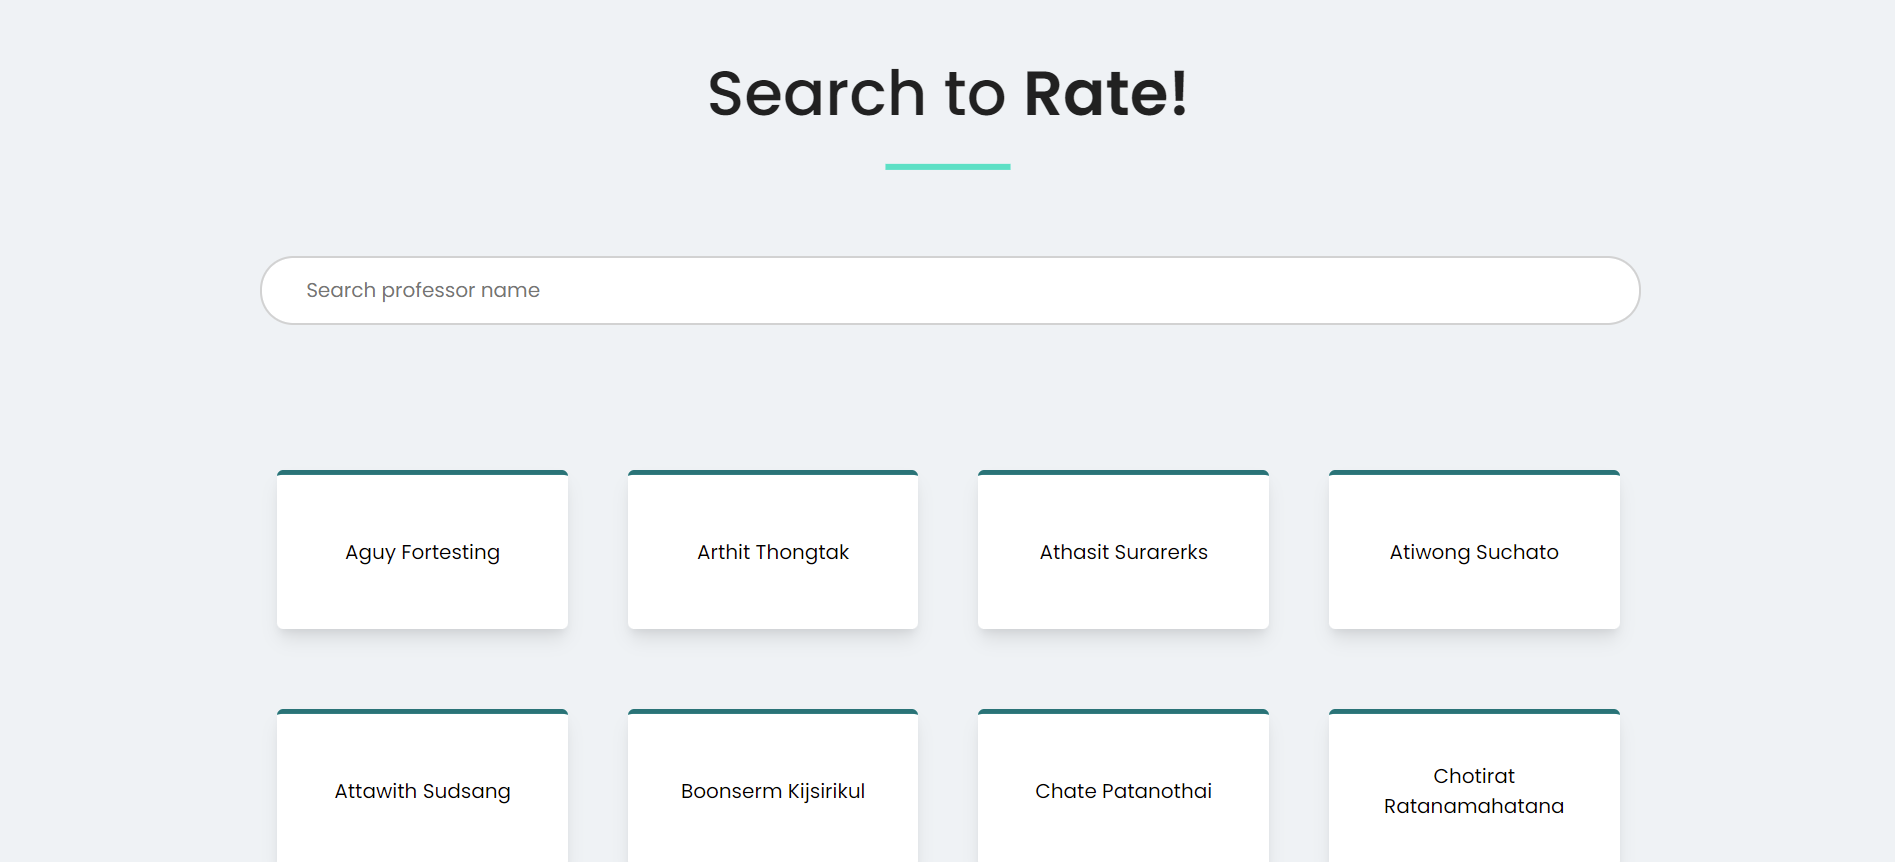
\includegraphics[scale=0.4]{proflist.png}
\end{center}
\par มีการใช้ navigation bar ที่ส่วนบนของหน้าเว็บ มี search box ที่จะกรองชื่ออาจารย์ทุกครั้ง\\
ที่ตัวอักษรในช่องค้นหาถูกเปลี่ยนแปลง มีส่วนกล่องชื่ออาจารย์ถูกดึงมาจาก database ของ firebase
ที่สามารถคลิกเพื่อเข้าสู่หน้ารวมคะแนนและความคิดเห็นของอาจารย์แต่ละท่าน

\subsection{หน้ารวมคะแนนและความคิดเห็นของอาจารย์แต่ละท่าน}

\begin{center}
    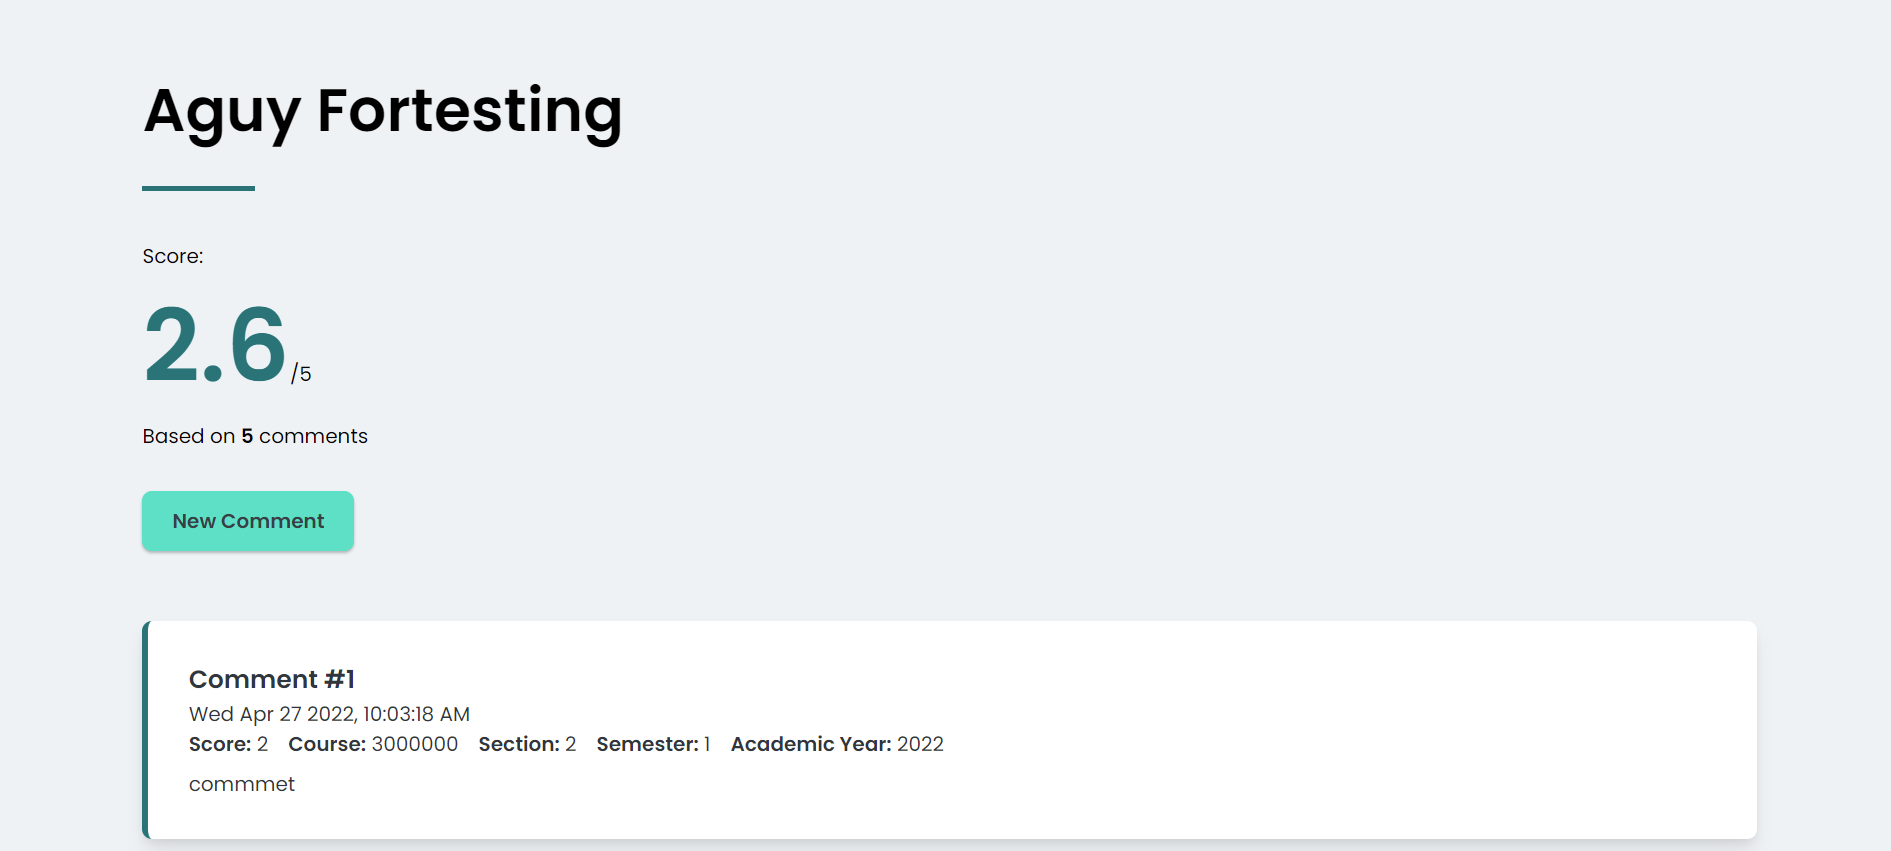
\includegraphics[scale=0.4]{professor_page.png}
\end{center}
\par มีการแสดงชื่ออาจารย์ท่านนั้นๆ มีส่วนการแสดงคะแนนเฉลี่ยและจำนวนความคิดเห็น ปุ่มกดเพื่อเพิ่มความคิดเห็น เพื่อเข้าสู้หน้าแสดงความคิดเห็น ในส่วนล่างมีกล่องความคิดเห็นเพื่อแสดงความคิดเห็นจากผู้เรียนที่เขียนไว้ก่อนหน้าถูกดึงมาจาก database ของ firebase
\par ส่วนบนยังมี navigation bar เหมือนหน้าหลัก
\pagebreak
\subsection{หน้าแสดงความคิดเห็น}
\begin{center}
    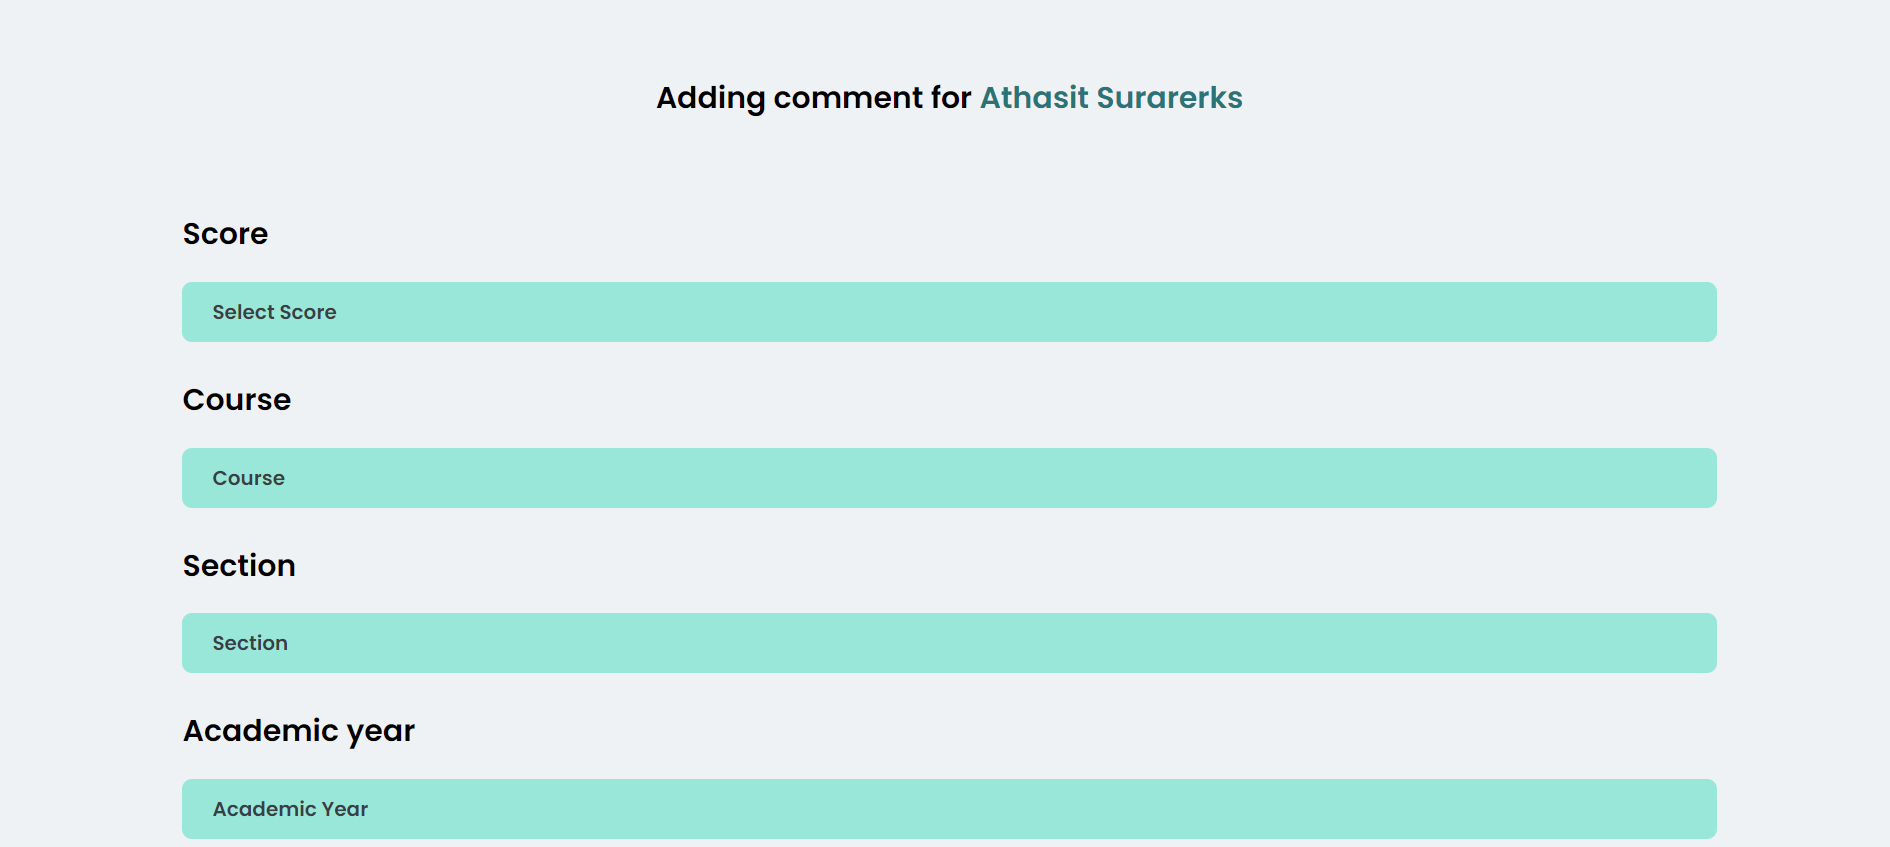
\includegraphics[scale=0.4]{add_comment.png}\\
    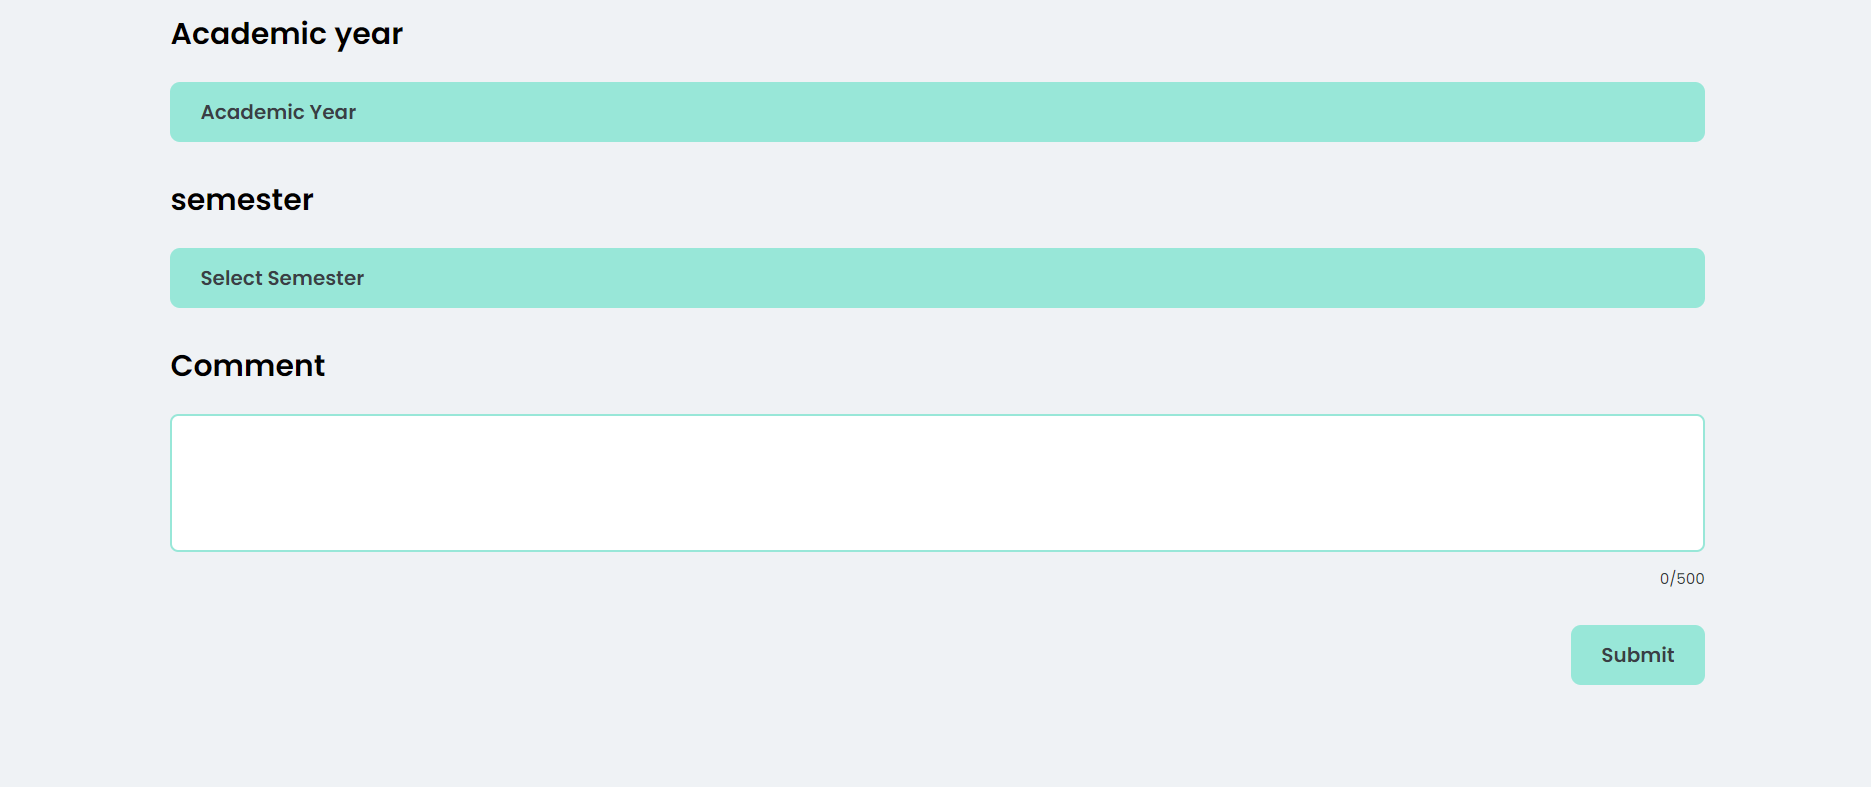
\includegraphics[scale=0.4]{add_comment2.png}
\end{center}

\par ส่วนบนมีการแสดงชื่ออาจารย์ที่กำลังถูกแสดงความคิดเห็น มีช่องสำหรับกรอกคะแนน รหัสวิชา ตอนเรียน ภาคเรียน ปีการศึกษา และช่องแสดงความคิดเห็นและมีปุ่ม submit เพื่อส่งข้อมูลที่กรอกไปยัง database เพื่อแสดงผลต่อไป
ในส่วนของหน้าเว็บเพจในการเข้าไปในหน้าอื่นนอกเหนือจากหน้าหลักจะมีการวาดหน้าเว็บใหม่บนหน้าเดิม เพื่อให้ถูกต้องตามวัตถุประสงค์ single-page web application
\section{Source Code}
Source Code ทั้งหมดสามารถเข้าถึงได้ที่ {\color{blue}\url{https://github.com/comp-eng-ess}}\\
Source Code สำหรับเว็บไซต์เข้าถึงได้ที่ {\color{blue}\url{https://github.com/comp-eng-ess/cp-rate-my-professor}}
\pagebreak
\section{Basic requirement}
\begin{itemize}
    \item The web application is a Single-page Web Application.
          \begin{itemize}
              \item เราทำ single-page web application ให้มีหลายหน้า \\(home, about, contact, รายละเอียดของอาจารย์แต่ละท่าน) โดยใช้ JavaScript วาด elements ในหน้าเดิม ไม่มีการ Refresh Page ระหว่างการใช้งาน
          \end{itemize}
    \item The web application help students with Online Learning (preferable in one specific aspect).
          \begin{itemize}
              \item ทางกลุ่มเราตกลงกันทำเว็บประเมินอาจารย์เพื่อสะท้อนความคิดเห็นของผู้เรียนต่ออาจารย์ โดยคาดหวังให้ผู้เรียนสะท้อนข้อดีและข้อเสียของการสอนในรูปแบบต่างๆของอาจารย์แต่ละท่านเพื่อทั้งตัวอาจารย์และบุคลากรที่เกี่ยวข้องสามารถนำข้อมูลไปปรับใช้หรือพัฒนาการสอน ผู้เรียนรุ่นต่อไปสามารถพิจารณาเข้าเรียนจากลักษณะการสอนของอาจารย์แต่ละท่านที่ตรงกับวิธีการเรียนของแต่ละคนได้
          \end{itemize}
    \item The front-end of the web application does NOT use any libraries/frameworks/plugins other than what was used in Activity 6.
          \begin{itemize}
              \item Frontend ใช้ HTML และ CSS พิ้นฐาน โดยไม่มีการใช้ Library เพิ่มเติม
          \end{itemize}
    \item The back-end of the web application does NOT use any libraries/frameworks/plugins other than what was used in Activity 7.
          \begin{itemize}
              \item Backend ใช้ Firebase Firestore และ Firebase Hosting โดยใช้ JavaScript ในการติดต่อกับ Database
          \end{itemize}
    \item All members contribute to the development and the contribution of each member is according to a "plan" agreed among the members of the group
          \begin{itemize}
              \item สมาชิกกลุ่มได้มีการวางแผนและแบ่งงาน มีการนัดประชุมเพื่ออัพเดทงานที่เหลือและสรุปความคืบหน้าตลอดช่วงการทำงาน
              \item รายละเอียดการวางแผนอยู่ที่ \textbf{\autoref{sec:plan}}
          \end{itemize}
\end{itemize}
\section{Challenging requirements}

\begin{itemize}
    \item The web application displays and interacts with the user nicely on different screen sizes and orientations.
          \begin{itemize}
              \item การออกแบบเว็บไซต์สำหรับแสดงผลในหน้าจอหลายขนาด เริ่มทำโดยออกแบบเว็บไซต์ที่ใช้บน PC ก่อน
              \item ไปปรับใช้ในการออกแบบของมือถือผ่านคำสั่ง @media (max-width: 480px) จากนั้นปรับ style ใน css ให้เหมาะกับมือถือในแต่ละรุ่นในขั้นตอนสุดท้าย
          \end{itemize}
    \item The application has a nice look and feel GUI.
          \begin{itemize}
              \item ในส่วนของการออกแบบหน้าเว็บของเราพยายามให้ Interface มีความเข้าถึงผู้ใช้ได้ดี และเข้าใจง่าย โดยเรามีการ Design ผ่าน Figma ก่อนมาทำใน css
              \item เมื่อ Coding จริงถ้าพบว่า Experiences ไม่ดีเท่าที่วางไว้แล้วนำมาคุยและปรับต่อ
          \end{itemize}
    \item The web application has a unique feature enhancing user experience
          \begin{itemize}
              \item มีการทดลองใช้งานจริงเพื่อหาข้อบกพร่องในการใช้งาน
              \item Design การทำงานต่างจาก Website ที่มีการ comment ทั่วไป โดยไม่ให้มีการลบ
              \item เน้น Privacy เป็นเป้าหมายสำคัญ
          \end{itemize}
\end{itemize}
\pagebreak
\section{ขั้นตอนการทำงาน}
\subsection{แผนการทำงาน}
\label{sec:plan}
\begin{center}
    \begin{tabular}{ | c | c |  }
        \hline
        งาน                              & ช่วงเวลาที่ดำเนินงาน                                       \\
        \hline
        \hline
        Initial Project Discussion       & \formatdate{12}{04}{2022} ถึง \formatdate{15}{04}{2022} \\
        Feature Planning                 & \formatdate{16}{04}{2022}                              \\
        UI Design                        & \formatdate{17}{04}{2022} ถึง \formatdate{19}{04}{2022} \\
        Backend Design                   & \formatdate{17}{04}{2022} ถึง \formatdate{19}{04}{2022} \\
        Backend and Frontend Development & \formatdate{19}{04}{2022} ถึง \formatdate{26}{04}{2022} \\
        Presentation and Report          & \formatdate{24}{04}{2022} ถึง \formatdate{27}{04}{2022} \\
        \hline
    \end{tabular}
\end{center}
\pagebreak
\subsection{หน้าที่รับผิดชอบ}
\begin{enumerate}
    \item Naphat Darunaitorn
          \begin{itemize}
              \item Project Manager - Assigning meetings, Assigning works to group member,
              \item Website Feature Design - Design the features that should be in the website and Creating draft UI in html
          \end{itemize}
    \item Noppakorn Jiravaranun
          \begin{itemize}
              \item Frontend Development - Creating css stylesheets for the website and Creation of UI Layout
              \item Backend Design - Design database schema and Handling the permission of using firebase
              \item Backend Development - JavaScript development with firebase
              \item Developer Experiences Improvement - Setting up GitHub with automatic firebase deployment, Merging Pull Request, Code Review
          \end{itemize}
    \item Nopparuj Poonsubanan
          \begin{itemize}
              \item Frontend Development - Creating css stylesheets for the website and Creation of UI Layout
              \item Backend Development - JavaScript development with firebase
          \end{itemize}
    \item Ittipat Yodprasit
          \begin{itemize}
              \item Frontend Design - Frontend Design in Figma and Beautiful UI Design
              \item Frontend Development - Creating css stylesheets for the website and Creation of UI Layout
          \end{itemize}
\end{enumerate}
\end{document}